
\subsection{Classical Spin Liquids} 

We have seen that frustrated and unfrustrated magnets have different microscopic order. However, in order to demonstrate that these host truly different phases one must consider their bulk properties. The simplest signature of frustration can be found by measuring the magnetic susceptibility $\chi$ of the material as a function of temperature \cite{ramirez_strongly_1994,mugiraneza_tutorial_2022}. In a conventional ferromagnet or antiferromagnet the system undergoes a `melting' phase transition as temperature in increased. At low temperature the spins are frozen in place, forming the (anti-)ferromagnetic ground state, however at some temperature $T_C$, the system undergoes a phase transition to a `liquid' phase in which the spins are able to fluctuate freely -- forming a paramagnetic phase. This transition can be approximately described using mean field theory \cite{simon_oxford_2013}. Here, the high-temperature susceptibility of the Hamiltonian in Eqn.~\ref{eqn:heisenberg_model} is given by
\begin{align}
    \chi^{-1} \sim T - \theta_{CW},
\end{align}
where the Curie-Weiss temperature $\theta_{CW}$ depends only on the microscopic couplings of the model. In the mean field approximation it is given by
\begin{align}
    \theta_{CW} = \frac 23 z S(S+1 ) J,
\end{align} 
where $z$ is the coordination number of a site in the lattice, and $J$ is the coupling strength. Considering the sign of $J$, we see that ferromagnetic systems have a positive Curie-Weiss temperature, whereas for anti-ferromagnets it is negative. In the absence of frustration, both the FM and AFM cases undergo a phase transition at temperature $T_C$ to a magnetically ordered phase --  in mean field theory we find that $T_c$ exactly equals $|\theta_{CW}|$, in real systems it is usually close but not exactly equal to it. This phase transition can be measured as kink or singularity in $\chi(T)$.

\begin{figure}
    \centering
    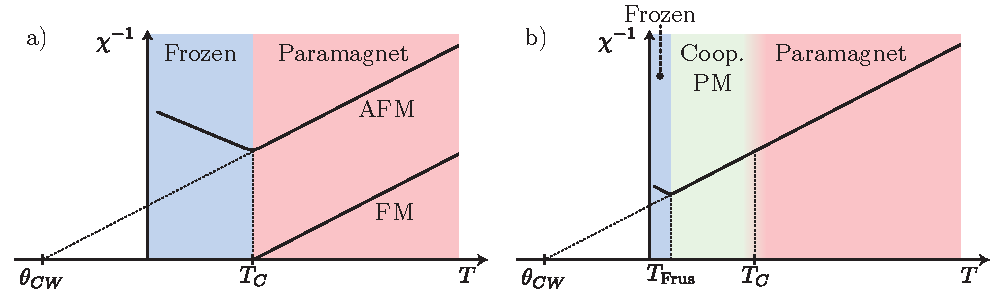
\includegraphics{introduction/figures/chi_t.pdf}
    \caption[Inverse magnetic susceptibility of a ferromagnet, antiferromagnet and frustrated antiferromagnet as a function of temperature.]{
        Inverse magnetic susceptibility plotted against temperature for a ferromagnet, antiferromagnet and frustrated antiferromagnet with the same value of $|\theta_{CW}|$. 
        In all three cases, the high temperature dependence is linear, indicating a disordered paramagnetic phase.
        \textbf{(a)}~In the ferromagnetic case the susceptibility diverges at temperatures below $T_C \sim \theta_{CW}$ indicating a magnetically ordered phase with bulk magnetization. 
        The antiferromagnetic system also undergoes an ordering transition at $T_C \sim \theta_{CW}$. Thus, the phase boundaries (indicated with colour) contain two phases, a high temperature paramagnetic phase and a low temperature frozen phase.
        \textbf{(b)}~In the frustrated antiferromagnet the ordering transition happens at a much lower temperature $T_{\textup{Frus}} \ll \theta_{CW}$. Between $T_C \sim - \theta_{CW}$ and the freezing temperature $T_{\textup{Frus}}$, the material forms a cooperative paramagnet phase, where thermal fluctuations are only able to explore the degenerate ground states and a small number of low-lying excited states.
        } 
    \label{fig:chi_t}
\end{figure}%
The story differs substantially when frustration is present. Here, the combination of a less energetically favourable ground state and abundance of degenerate ground states serves to suppress magnetic ordering. Thus, in systems where a freezing transition does occur, the transition temperature is much lower than the scale set by $\theta_{CW}$, this is shown in Fig.~\ref{fig:chi_t}b. In the interval between $T_{Frus}$ and $T_C$, the frustrated system enters a different phase to the conventional para- or ferromagnetic phases. Here, fluctuations remain that explore the degenerate set of ground states (and low-lying excitations around it), but are prohibited from exploring the full space of spin-configurations in the way that a high-temperature paramagnet might be able to. This `cooperative paramagnet' phase is thus highly dependent on the specifics of the material -- which define the states that can be explored -- in contrast to the $T>T_C$ paramagnetic phase, which is generic to all paramagnets. 

The question remains, however, whether the cooperative paramagnet phase is truly distinct from a traditional paramagnet. That is, does the restriction to fluctuate only around a specific low-energy subspace lead to any measurable long-range consequences? In general, the answer to this question depends on the specifics of the system. Thus, let us provide a simple example -- that of spin ice -- where the answer is yes. In particular, we shall see that the local constraints in this model lead to the emergence of a classical \textit{spin liquid} phase \cite{castelnovo_magnetic_2008,castelnovo_spin_2012,balents_spin_2010}. Although this term lacks a formal definition, it is broadly accepted that to qualify as a spin liquid, two connected properties that be present: fractionalised excitations and an emergent gauge field \cite{savary_quantum_2017,knolle_field_2019}.

In a fractionalised system, the quasiparticles carry a fraction of the properties of the constituent particles in the material. The most famous example of this phenomenon is the fractional quantum Hall effect \cite{laughlin_nobel_1999}, where the quasiparticles carry a fraction of the charge (and a fraction of the exchange statistics) of the electron. In a magnetic material the natural excitations are spin flips -- a dipole-like excitation. As we shall see in the following example, these dipoles can fractionalise into a pair of magnetic monopoles, which are then free to propagate independently throughout the material, behaving as particles in their own right. Of course, even in a fractionalised material, one must respect the conservation laws implied by the original, unfractionalised constituents. That is, quantities such as the total charge, or the total magnetic moment of the system are not allowed to take fractionalised values. In a quantum Hall system where excitations have $\frac pq$ charge, we must ensure that the system always contains a multiple of $q$ such particles. Similarly, monopoles in spin ice must always be created and destroyed in pairs, else the system as a whole will have nonzero magnetic charge, which is forbidden in electromagnetism. This global constraint means that an effective description of the system must include an emergent gauge field, whose rose is to enforce this symmetry, encoding the constraint locally in the configuration of the field. 

\subsubsection{Fractionalisation in Spin Ice}

We now illustrate a simple toy model for spin ice, demonstrating the way that fractionalised excitations can emerge in a classical system. The study of spin ice is an enormous field, and we shall provide only enough detail to build an intuitive picture for understanding the monopole nature of the excitations, however for a thorough discussion see the following Refs.~\cite{castelnovo_magnetic_2008,castelnovo_spin_2012,udagawa_spin_2021}.

The model is constructed on the pyrochlore lattice formed by corner-sharing tetrahedra, shown in Fig.~\ref{fig:frustrated_simplex}c. The arrangement of tetrahedra on this lattice is bipartite, and we shall label the two sets of tetrahedra with $A$ and $B$, where every spin connects between one tetrahedron on each sublattice. At each site is a single magnetic moment. In real spin-ice compounds such as Dy$_2$Ti$_2$O$_7$ or Ho$_2$Ti$_2$O$_7$ the magnetic moments have $S = 15/2$ and $8$ respectively. Thus, to a good approximation they can be treated as classical degrees of freedom. Spins interact with one another through a ferromagnetic, dipolar coupling.
However, they are also subject to an extremely strong local anisotropy that confines each spin to point either directly into the tetrahedron or directly out \cite{bramwell_spin_2001}. Thus, we may model each spin with an effective Ising degree of freedom $\sigma_j = \pm 1$, according to
\begin{align}
    \textbf{s}_j = S \sigma_j \hat {\textbf n}_j,
\end{align}
where the unit vector $\hat {\textbf n}_j$ points from the $A$ tetrahedron into the $B$ tetrahedron. With this parametrisation, we see that the ferromagnetic Heisenberg coupling becomes an effective antiferromagnetic coupling in these Ising variables,
\begin{align}
    H = -\sum_{\braket{jk}} \textbf{s}_j \textbf{s}_k 
    \rightarrow 
    +\frac{S^2}{3}\sum_{\braket{jk}} \sigma_j \sigma_k,
\end{align}
where we have used the fact that for any two adjacent sites, $ \hat {\textbf n}_j \cdot  \hat {\textbf n}_k = 1/3$. As we did for the Heisenberg model (Eqn.~\ref{eqn:total_spin_trick}), this Hamiltonian can be re-expressed as sum of the total spin on each tetrahedron,
\begin{align} \label{eqn:ice_rules}
    H = \frac{S^2}{6} \sum_{\textup{tet.}} 
    \bigg |
    \sum_{j \in\tetrahedron} \sigma_j
    \bigg |^2 + \textit{constant}.
\end{align}
Thus, we see that the energy for every tetrahedron is minimised so long as two of its constituent spins point in, and two point out, as shown in Fig.~\ref{fig:spin_ice}a, this condition is known as the material's \textit{ice rules}. 

\begin{figure}
    \centering
    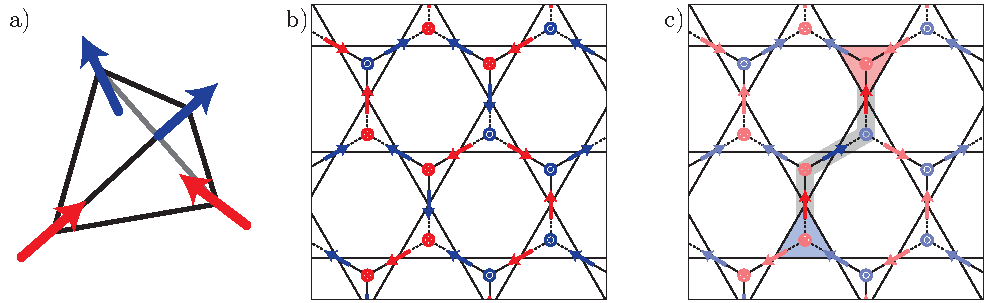
\includegraphics{introduction/figures/spin_ice.pdf}
    \caption[Ice rules, spin ice ground state and the creation of a pair of monopoles.]{
            \textbf{(a)}~A single tetrahedron in the ground state, where the two red moments point into the tetrahedron, and the two blue moments point out.
            \textbf{(b)}~A diagram of a ground state configuration on a single layer of tetrahedra, forming a slice of the three-dimensional pyrochlore lattice. Here the solid tetrahedra extend up `out of the page', whereas the dashed tetrahedra extend down `into the page'. Each of these sets of tetrahedra connect to the other layers of the lattice, and we label them with $A$ and $B$. Spins are coloured with red if they point into an $A$-type tetrahedron, and blue if they point out of it, with spins that point in or out of the page indicated with $\otimes$ or $\odot$ depending on orientation. Thus, as long as each tetrahedron connects to two red and two blue spins, it is in the ground state.
            \textbf{(c)}~A section of the ground state from subplot (b) is shown, however now we flip a single spin (highlighted in grey). This has the effect of creating one tetrahedron that has three spins pointing out, acting as a source of magnetic flux (highlighted in blue), and one that has three spins pointing in, acting as a sink (highlighted in red).
            \textbf{(d-e)}~By flipping successive spins it is possible to separate the two ends of the dipole, effectively producing a pair of monopole excitations which are free to propagate independently through the material. Connecting these monopoles is a grey Dirac string, consisting of the line of spins that has been flipped with respect to the ground state. 
        } 
    \label{fig:spin_ice}
\end{figure}%

As we have seen many times by this point, this frustration leads to the formation of an extensively degenerate ground state. Each tetrahedron has 16 possible configurations of the four spins, 6 of which are in the ground state. Thus, a lattice containing $N_s$ spins and $N_t = N_s/2$ tetrahedra will have $2^{N_s}$ total spin configurations, of which around 
\begin{align}
    2^{N_s} \left ( \frac 6{16}\right )^{N_t}
\end{align}
are in the ground state. One example of such a ground state is depicted in Fig.~\ref{fig:spin_ice}b.

On this background, a low-lying excited state can be created by flipping a single spin. Before this flip, the two adjacent tetrahedra were in the ground state, with two in-spins and two out-spins. After the flip this is no longer the case. Now one tetrahedron has three spins pointing in, and the other has three spins pointing out. Thus, the pair of tetrahedra collectively resemble a single dipole, with the three-out tetrahedron acting as a source of flux, and the three-in tetrahedron acting as a sink, this is shown in Fig.~\ref{fig:spin_ice}c. This is not yet surprising, since a spin flip can always be seen as creating a dipole on a neutral background. However, the fractionalised nature of spin ice is revealed by performing further spin flips to separate the two constituent monopoles forming this dipole. This is shown in Fig.~\ref{fig:spin_ice}d and \ref{fig:spin_ice}e, where we see that it is always possible to return a tetrahedron to being magnetically neutral, at the cost of creating another three-in or three-out tetrahedron adjacent to it. 

Thus, we see that a dipole excitation in spin ice can be separated into a pair of monopoles, each corresponding to a tetrahedron with an unequal number of spins pointing in and pointing out. Each monopole costs a fixed amount of energy to create, defined according to Eqn.~\ref{eqn:ice_rules} as $E_{mp} = S^2/3$. Furthermore, in our nearest-neighbour model, once this energy penalty has been paid, the monopoles are completely deconfined, since we can freely move them around with successive spin-flips at no extra cost.\footnote{Note that this is not the case in real spin ice materials. In a more accurate model, one would have to take into account longer-ranged dipolar interactions rather than only considering nearest neighbours as we have done here. In this case, the monopole excitations behave analogously to electrical point charges, with to a (magnetic) coulomb interaction \cite{castelnovo_spin_2012}. However, they remain deconfined, since under such a potential one pays a finite energy cost to infinitely separating a pair of monopoles.}

Starting with a single realisation of the ground state, any monopoles we create are connected by a `Dirac string' of spins that have been flipped with respect to the initial state. Thus, we note that a single monopole can never be created as the result of a local operation, since one must always flip the entire string, and another monopole will be created at the other end. This condition takes care of the condition that monopoles must appear in pairs. However, these Dirac strings are only observable provided we know exactly which ground state we started in. In a system at finite temperature the Dirac strings are unobservable, as thermal fluctuations mean that no single initial ground state can be identified. It is possible, however, to observe the Dirac string if we include a perturbation that breaks the degeneracy of the ground state. This can be done for example by including a weak magnetic field, selecting a lowest-energy configuration of spins for each tetrahedron \cite{morris_dirac_2009}. However, this comes at a price, since now the Dirac strings come with an energy cost that scales linearly with string length, meaning that the monopoles cannot be infinitely separated without paying an infinite energy cost, and so are no longer deconfined.


\subsubsection{Quantum Spin Liquids}

\subsubsection{Breaking a Spin Liquid}

\todo{Final paragraph on how the enemy of the spin liquid is disorder/ perturbations/ order-by-disorder -- i.e. these effects ruin the incredibly even-handed superpositions necessary for fluctuations to explore these ground states}
